\chapter{Modelling Larval Stage in a Vial}
 Competition for food during larval stage is determined by not only larval density but also ecological factors inside a food vial such as nitrogenous waste build up (ref), diffusion of waste in the food below (ref), total food amount (ref). Thus, in order to investigate the adaptation to larval crowding, it is crucial to understand the ecology of the vial in which larval stage of Drosophila lab populations is maintained and replicating such environment during larval feeding becomes the first step in modelling the larval growth. Previous experimental studies on Drosophila in laboratory conditions, have shown the pattern of the growth of larvae, excretion of nitrogenous waste, larval feeding behavior in response to the waste excreted, development time (ref). Based on these experimental studies, I have created an individual-based model which considers feeding rate, efficiency to convert food into biomass, critical size and waste tolerance as larval trait parameters to measure other traits which are variables such body size, development time, and survivorship.
\section{Ecology of a Vial in Drosophila Cultures}
During larval feeding inside a vial, larvae are able to access only a certain amount of food from the total food available at a given time point. This is due to their inability to dig more to access food (ref), and this accessible food is referred as the feeding band. For simplicity, feeding band is taken as volume of food proportional to the diameter of the vial. In the model, I also assume this feeding band to be a constant volume of food in all types of culture vials till it reaches the bottom of the vial. The growth of larvae in the model is affected by waste build up and food quality in the feeding band. I also consider a diffusion band which is a part of the total food below feeding band where some amount of waste can diffuse from feeding band at each time step. Fig ~\ref{fig:vial} is the visualization of feeding band and diffusion band during larval feeding.

\begin{figure}[h]
  \centering
  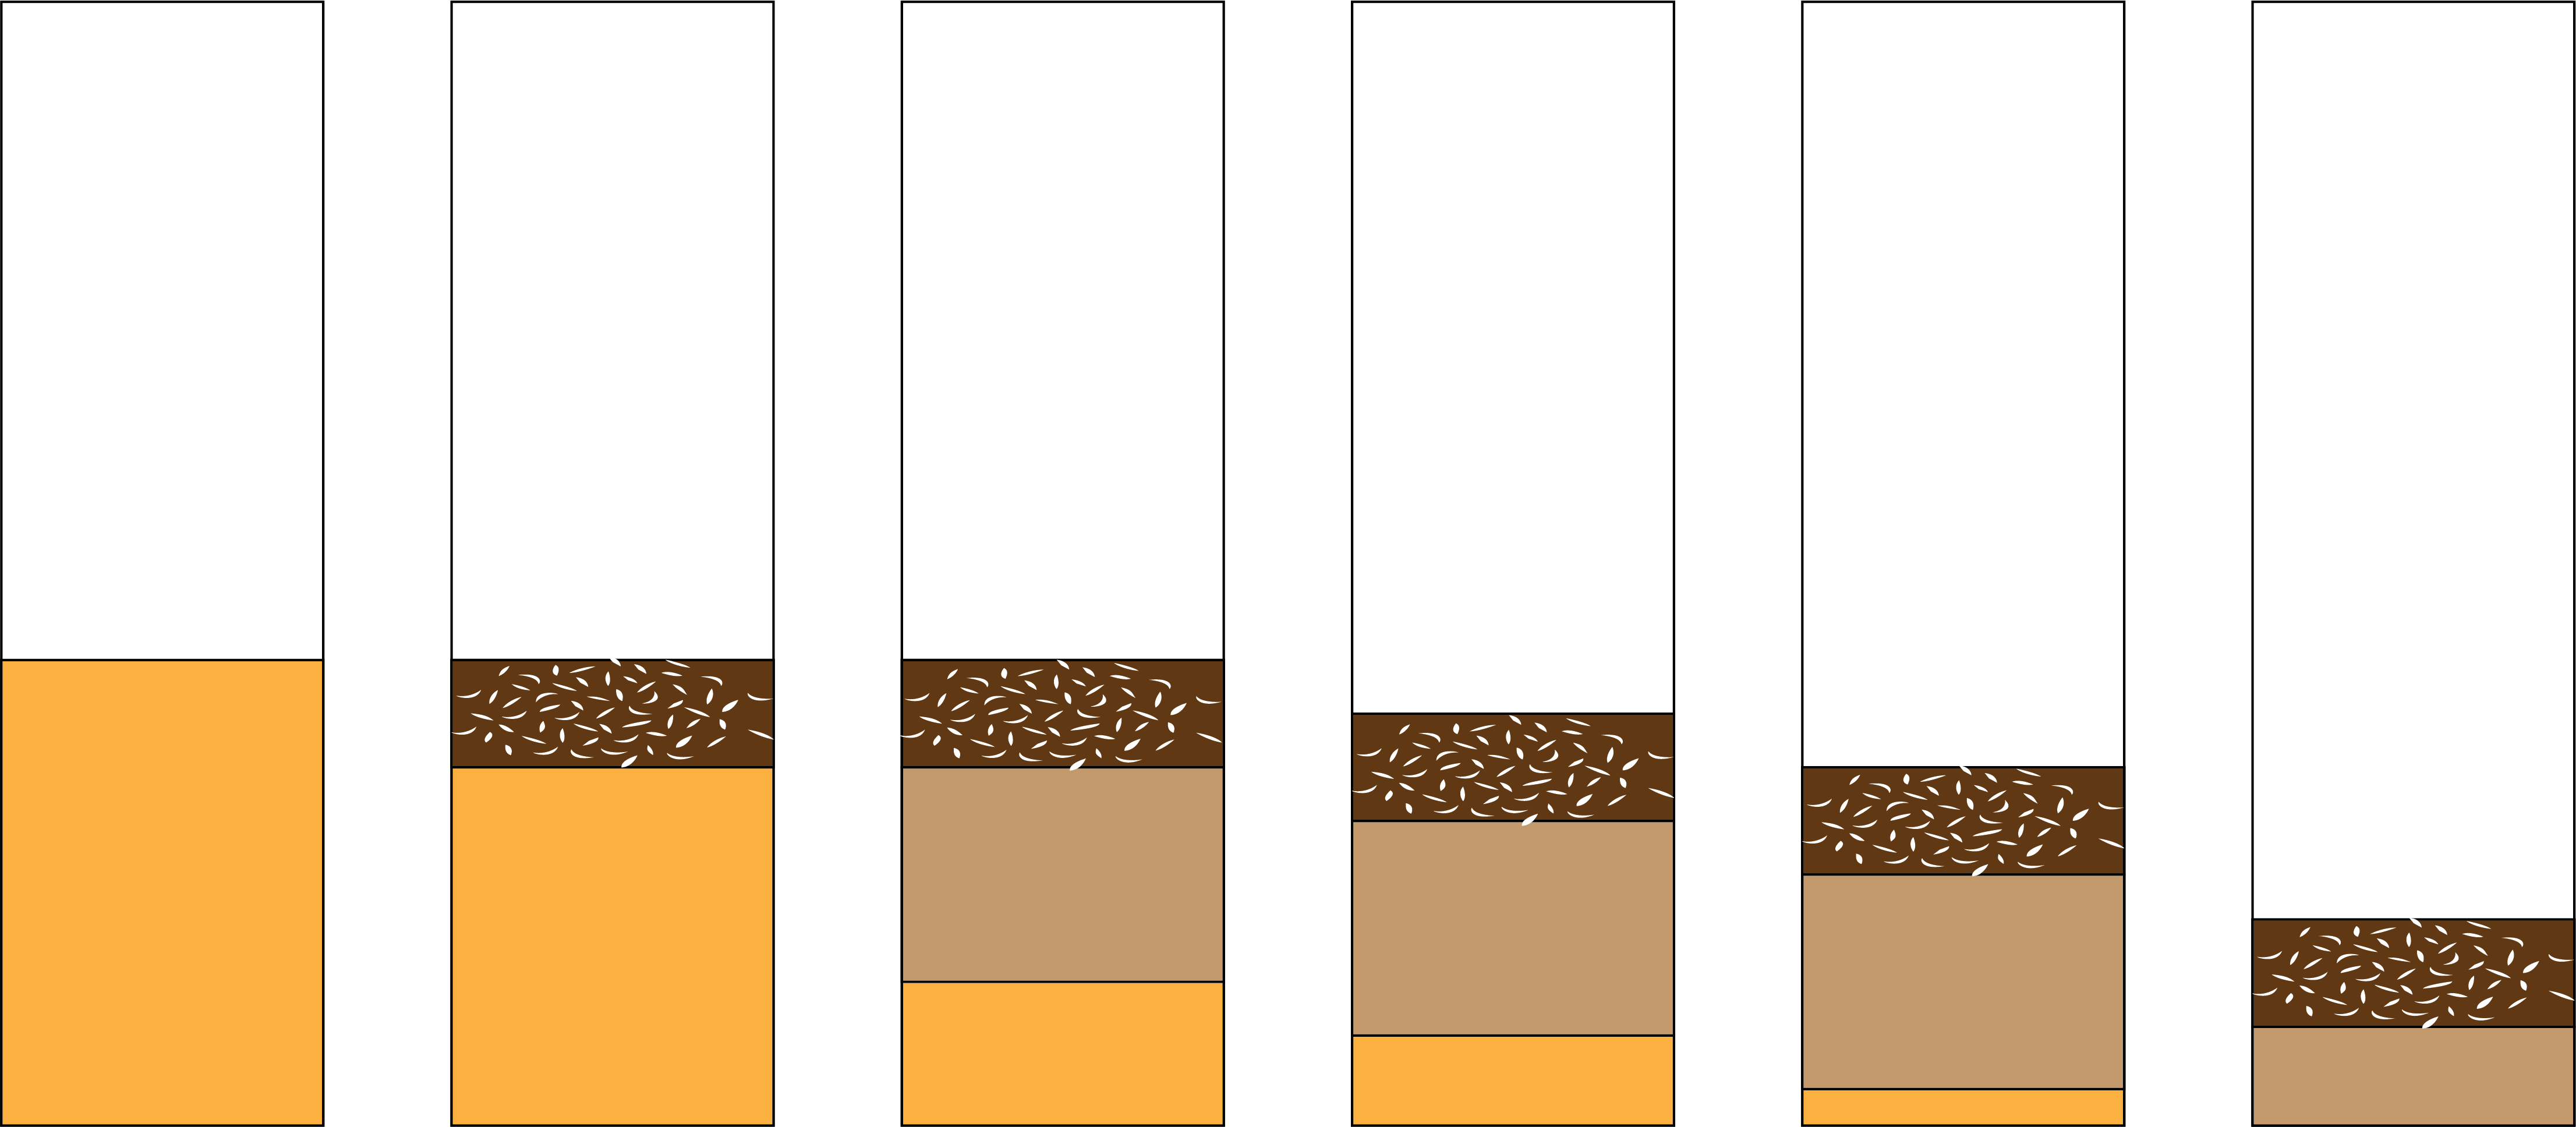
\includegraphics[width=0.75\textwidth]{C2/Figs/vial_diagram}
  \caption{Ecological dynamics in a vial during larval feeding}
  \label{fig:vial}
\end{figure}

\section{Larval Stage Model}
Each individual egg is assigned larval trait parameters from respective distributions with certain mean and variation (table no.). For a given amount of food and number of eggs keeping the sex ratio 1:1, the model follows certain set of rules as described in fig ~\ref{fig:larval_model} which are simulated in discrete time steps. Critical size and efficiency are taken as sexually dimorphic traits and are assigned depending on the sex of the individual larva. Critical size and efficiency of females are assumed to be higher than that of males.\\ \\
The inital size of all larvae is same and the growth is determined by larval trait parameters such as initial feeding rate, efficiency, waste tolerance and critical size assigned to each individual from distributions with respective mean trait value and variation. The larval growth is divided into two stages determined by whether critical size is reached or not, These stages are called pre-critical and post-critical stage. \\
In pre-critical stage of the larva, feeding rate is a linear function of time, given as:
\[Fr_{i}(t) = fr_{i} + x_{1}\cdot t\]
Here, \\
$fr_{i}$: initial feeding rate of $i^{th}$ larva; $x_{1}$: scaling parameter, \\
$t$: given time step; $Fr_{i}(t)$: Feeding rate at time $t$

\begin{figure}[h]
  \centering
  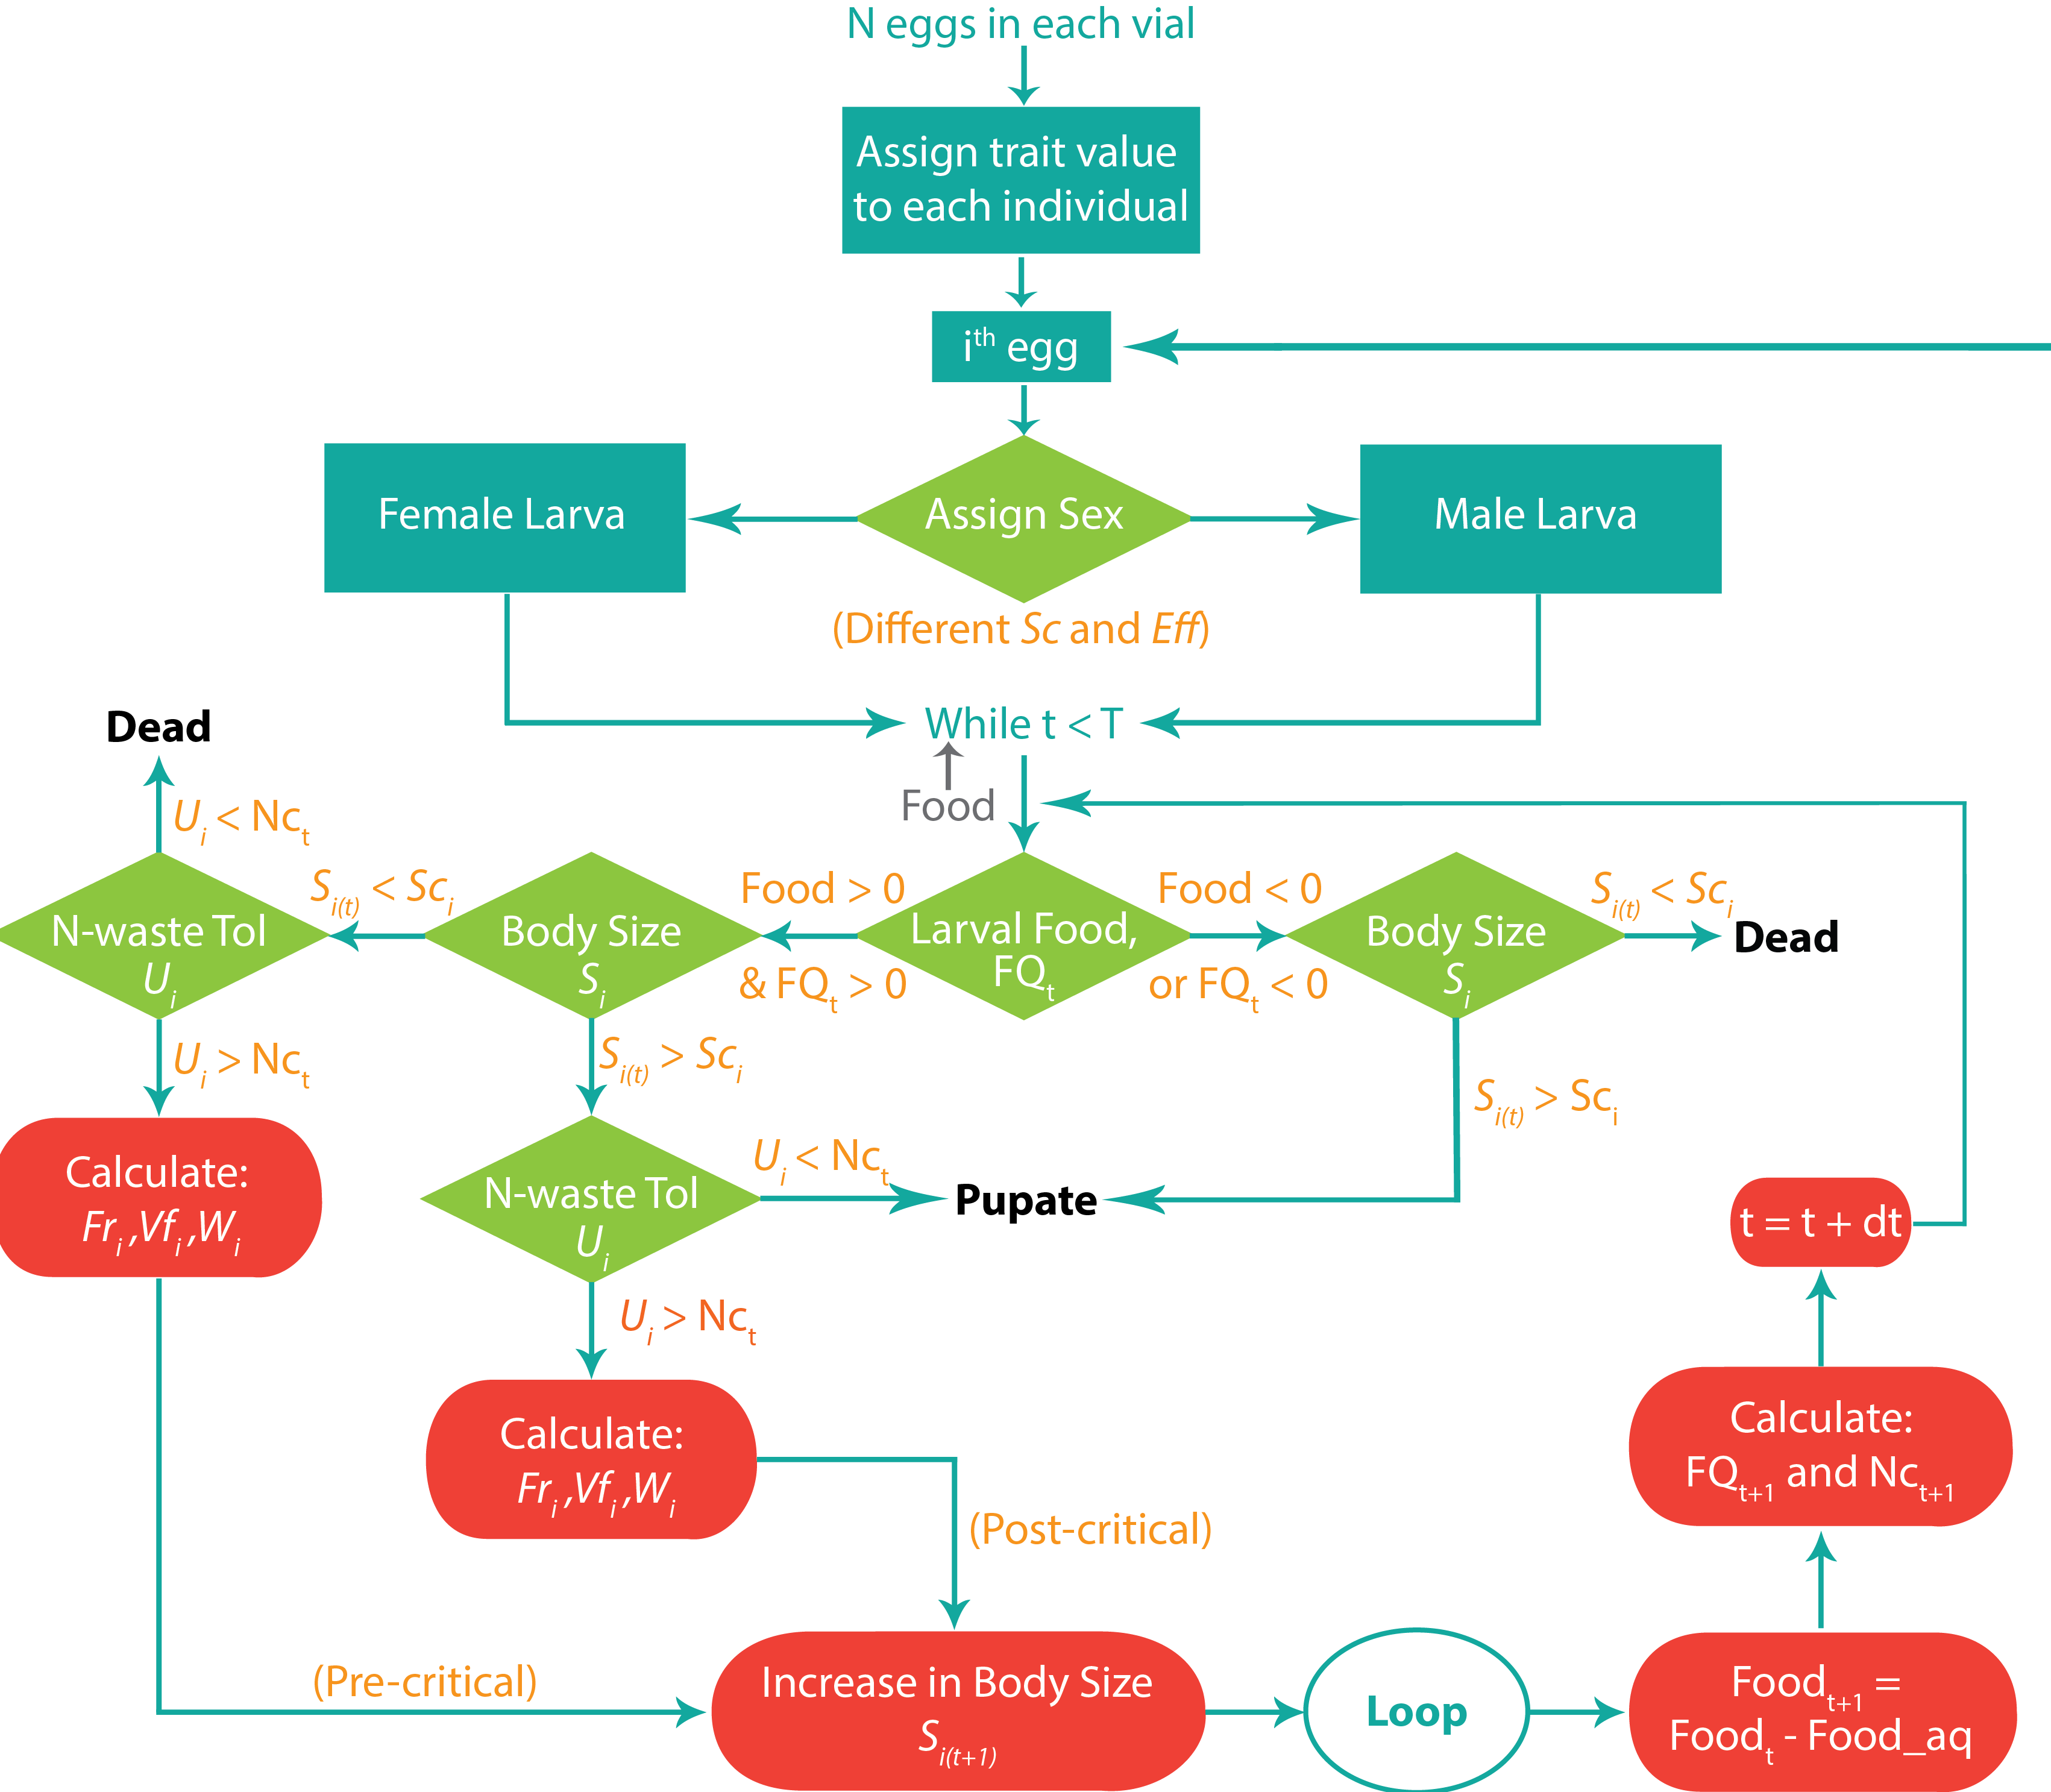
\includegraphics[width=0.8\textwidth]{C2/Figs/larval_model}
  \caption{Flowchart of the larval stage in the model}
  \label{fig:larval_model}
\end{figure}

Feeding rate stays constant During post-critical stage. During pre-critical growth Volume of food taken in one bite is taken as constant $V_{f}(pre)$ and during post-critical growth it is $V_{f}(post) = 1.5\cdot V_{f}(pre)$. Food consumed by all larvae at time step $t$ is given as:
\[FoodEaten(t) = \sum_{i}food\_eaten_{i}(t) = \sum_{i}Fr_{i}(t)\cdot V_{f}\]
The increase in body size at time $t$ is $S_{i}(t+1)$ and give as:
\[S_{i}(t+1) = S_{i}(t) + food\_eaten_{i}(t)\cdot \epsilon_{i}\cdot FQ_{fb}(t)\]
Here,\\
$\epsilon_{i}$: Efficiency to convert food eaten into biomass of $i^{th}$ larvae,\\
$FQ_{fb}(t)$: Food quality of the feeding band at time $t$ \\
After feeding and utilizing food consumed at given time step, larva produces nitrogenous waste $waste\_prod_{i}(t)$. This affects the total waste produced by all the larvae after feeding:
\[WasteProd(t) = \sum_{i}waste\_prod_{i} = \sum_{i}[food\_eaten_{i}(t)\cdot (1-\epsilon_{i}\cdot FQ(t))]\]
Based on this waste produced, total waste accumulated till time step $t$ in feeding band and diffusion band is calculated considering $k_{d}$ proportion of waste in the feeding band diffuses into diffusion band at each time step.
\[Waste_{fb}(t+1) = Waste_{fb}(t) + (1-k_{d})\cdot WasteProd(t) + \frac{FoodEaten(t)\cdot Waste_{db}}{dband}\]
\[Waste_{db}(t+1) = Waste_{db}(t) + k_{d}\cdot WasteProd(t) - \frac{FoodEaten(t)\cdot Waste_{db}}{dband}\]
Food quality of the feeding band at time step $t$ is:
\[FQ_{fb}(t) = 1 - \frac{Waste_{fb}(t)}{fband}\]
If $FQ_{fb}(t) \leq 0 $, it means that there is no food available to eat and feeding band contains only nitrogenous waste and larvae stop eating.\\
$k_{d}$ is dependent on the food available in the vial and determines whether waste is diffused into the diffusion band. Its values are assigned at each time step as follows:
\begin{enumerate}[i]
  \item $k_{d}$ is a constant $> 0$ if $food > fband+dband$
  \item $k_{d} = 0$ if $food \leq fband+dband$
\end{enumerate}
Each larva feeds and increase the body size in each time step based on the conditions for food available ($food$), food quality ($FQ(t)$), critical size ($sc_{i}$) and waste tolerance ($u_{i}$) described in fig ~\ref{fig:larval_model}.\\
Values for larval trait parameters obtained from distributions as described in table (ref), were varied and calibrated to obtain survivorship, body size and development time results similar to the empirical results in various larval densities (table no.). These larval trait values represent MB-tpye (control population) larval traits.

\newpage
\section{Feeding Band Dynamics}
Simulations are performed for MB-type larvae to observe the waste build up dynamics in a food vial with different larval densities during larval feeding. In fig ~\ref{fig:waste}, waste build in the feeding band throughout larval feeding at different larval densities is plotted. At low density i.e. 60 eggs / 6 ml food (MB culture), there is very little nitrogenous waste building up due to diffusion and plenty of food available below the feeding band at all time steps unlike at high densities. \\
\begin{figure}[h]
  \centering
  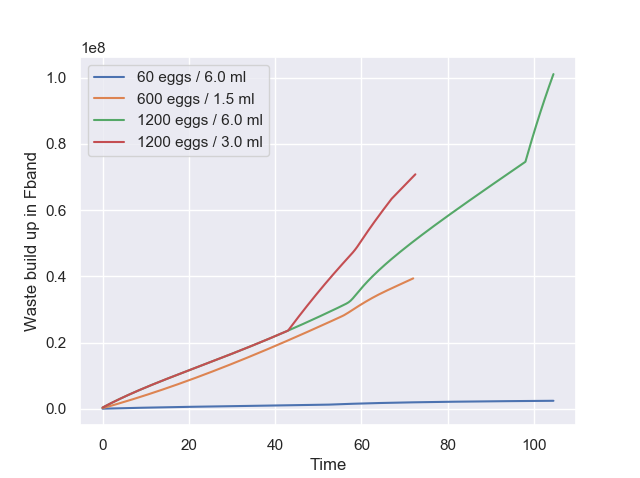
\includegraphics[width=0.8\textwidth]{C2/Figs/waste build up}
  \caption{Waste build up in the feeding band}
  \label{fig:waste}
\end{figure}\\

High densities - 600 eggs / 1.5 ml food (MCU culture) and 1200 eggs / 3 ml food (CCU culture) show different patterns of waste build up in the feeding band, even though total larval density is equal. This is due to differences in diffusion pattern in MCU and CCU culture vials. In MCU culture vial, there is very little food available below the feeding band, thus diffusion does not occur and waste build in the feeding band increases gradually. In CCU culture vial, waste build is almost in same qauntity as in MCU culture in earlier stage, even though effective larval density is double (number of larvae per feeding band). This is due to the availablilty of food below feeding band in CCU culture where waste can diffuse. After approx. $40^{th}$ time step, diffusion stops and waste from diffusion band enters feeding band in more quantity, thus giving a sudden increase in the waste build rate. \\ \\
LCU culture vial (1200 eggs in 6 ml food) also shows pattern waste build in the feeding band similar to CCU culture vial, but shows increase in the rate of waste build up at approx. $60^{th}$ time step as there is more food available below the feeding band compared to CCU culture vial. At approx. $100^{th}$ time step in LCU culture vial shows even more increase in the rate of waste build because diffusion band touches the bottom and starts shrinking.

\section{Discussion}
Time to reach critical size ~ survivorship ~ ccu and mcu differences
\pagebreak
\renewcommand\bibname{{References}}
\bibliography{References}
\bibliographystyle{plain}
